\section{Результати роботи та аналіз оптимальних умов роботи алгоритмів}
У роботі реалізовані такі модулі:
\begin{enumerate}
	\item train\_from\_folder - модуль навчання байесовського класифікатора з вказаної папки, в ній мають міститися кольорові фотографії та маски для кожної відповідно. Назви мають бути формату [номер]\_i.[формат] для зображення, та [номер]\_m.[формат] - маска;
	\item train\_from\_realsense - модуль навчання байесовського класифікатора за допомоги камери Intel Realsense.
	\item process\_opencv - обробка відеопотоку за допомоги байесовського класифікатора та отримання відео за допомоги бібліотеки opencv. Бібліотека opencv накладає деякі обмеження на максимальну кількість фреймів за секунду, тому було вирішено реалізувати варіант з використанням драйвера Intel Realsense так як в ньому такого обмеження немає;
	\item process\_realsense - обробка відеопотоку за допомоги байесовського класифікатора та отримання відео за допомоги драйвера Intel Realsense;
	\item show\_model\_representation - модуль, що призначений для читання байесовської моделі з файла та виведення зображень ілюстрацій навчання;
	\item filter\_model - модуль для роботи з моделями, в якому реалізовані усі зазначені у практичній частині перетворення матриці ймовірностей.
\end{enumerate}

Усі програмні модулі виконані у консольному середовищі з виведенням відеопотоків в окремі вікна для ілюстрації роботи алгоритмів.
\subsection{Віднімання фону}
Віднімання фону достатньо показало достатньо непогані результати.

\begin{figure}[H]
	\centering
	\begin{subfigure}[b]{0.45\textwidth}
		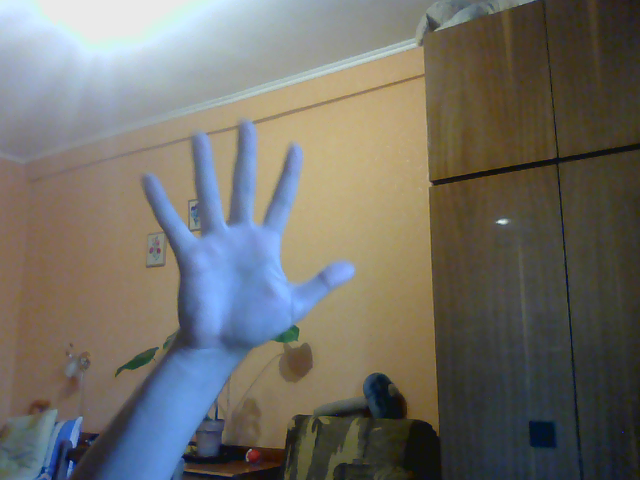
\includegraphics[width=\textwidth]{practise/img/hand1}
		\caption{Поточне кольорове зображення}
	\end{subfigure}
	\hfill
	\begin{subfigure}[b]{0.45\textwidth}
		
\includegraphics[width=\textwidth]{practise/img/mask1}
		\caption{Маска виділеного переднього плану}
	\end{subfigure}
	\caption{Ілюстрація роботи алгоритма віднімання фону}
	\label{fig:background_subtraction1}
\end{figure}

Значення першого критерія - 91.37%

Значення другого критерія - 0.03%

\begin{figure}[H]
	\centering
	\begin{subfigure}[b]{0.45\textwidth}
		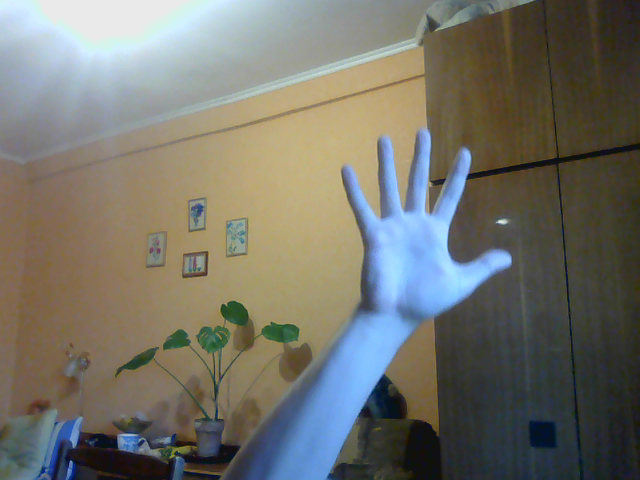
\includegraphics[width=\textwidth]{practise/img/hand2}
		\caption{Поточне кольорове зображення}
	\end{subfigure}
	\hfill
	\begin{subfigure}[b]{0.45\textwidth}
		
\includegraphics[width=\textwidth]{practise/img/mask2}
		\caption{Маска виділеного переднього плану}
	\end{subfigure}
	\caption{Ілюстрація роботи алгоритма віднімання фону}
	\label{fig:background_subtraction2}
\end{figure}

Значення першого критерія - 98.26%

Значення другого критерія - 0.74%

\subsection{Байесовський класифікатор}
\jointitles
\subsubsection{Класична реалізація}
Після навчання класифікатора можна отримати графічне представлення матриці ймовірностей як два зображення градації сірого.
\begin{figure}[H]
	\centering
	\begin{subfigure}[b]{0.45\textwidth}
		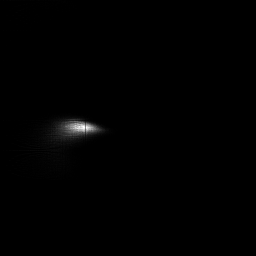
\includegraphics[width=\textwidth]{practise/img/b_start}
		\caption{Матриця ймовірностей}
		\label{fig:b_start}
	\end{subfigure}
	\hfill
	\begin{subfigure}[b]{0.45\textwidth}
		
\includegraphics[width=\textwidth]{practise/img/b_start_gen}
		\caption{Матриця ненульових ймовірностей}
		\label{fig:b_start_gen}
	\end{subfigure}
	\caption{Результат навчання класифікатора}
	\label{fig:bayesian_representation_start}
\end{figure}

На Рис. \ref{fig:b_start} показана матриця ймовірностей в градації сірого. Ймовірності переводяться методом домноження їх на 255. На Рис. \ref{fig:b_start_gen} показані усі елементри матриці ймовірностей, що мають ненульові значення.

\begin{figure}[H]
	\centering
	\begin{subfigure}[b]{0.45\textwidth}
		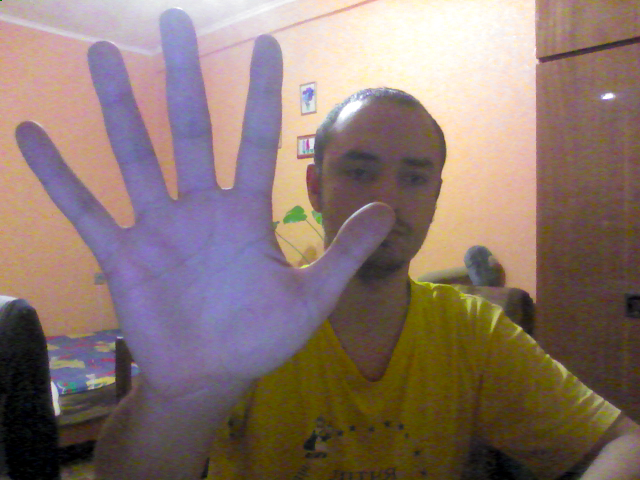
\includegraphics[width=\textwidth]{practise/img/b_color1}
		\caption{Кольорове зображення}
	\end{subfigure}
	\hfill
	\begin{subfigure}[b]{0.45\textwidth}
		
\includegraphics[width=\textwidth]{practise/img/b_mask1}
		\caption{Відфільтроване}
	\end{subfigure}
	\caption{Ілюстрація роботи байесовського класифікатора}
	\label{fig:bayesian1}
\end{figure}

Значення першого критерія - 84.62%

Значення другого критерія - 4.68%

\begin{figure}[H]
	\centering
	\begin{subfigure}[b]{0.45\textwidth}
		
\includegraphics[width=\textwidth]{practise/img/b_color2}
		\caption{Кольорове зображення}
	\end{subfigure}
	\hfill
	\begin{subfigure}[b]{0.45\textwidth}
		
\includegraphics[width=\textwidth]{practise/img/b_mask2}
		\caption{Відфільтроване}
	\end{subfigure}
	\caption{Ілюстрація роботи байесовського класифікатора}
	\label{fig:bayesian2}
\end{figure}

Значення першого критерія - 76.21%

Значення другого критерія - 3.84%

\subsubsection{Корекція класифікатора}

Застосувавши корекції ймовірностей матриця ймовірностей прийняла такий вид:
\begin{figure}[H]
	\centering
	\begin{subfigure}[b]{0.45\textwidth}
		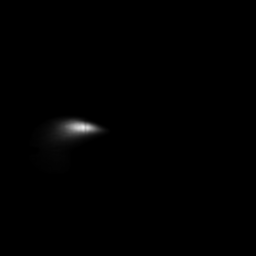
\includegraphics[width=\textwidth]{practise/img/b_end}
		\caption{Матриця ймовірностей}
		\label{fig:b_end}
	\end{subfigure}
	\hfill
	\begin{subfigure}[b]{0.45\textwidth}
		
\includegraphics[width=\textwidth]{practise/img/b_end_gen}
		\caption{Матриця ненульових ймовірностей}
		\label{fig:b_end_gen}
	\end{subfigure}
	\caption{Результат обробки матриці ймовірностей класифікатора}
	\label{fig:bayesian_representation_end}
\end{figure}

Значення першого критерія покращились майже на 3\%. Значення другого критерія практично не змінилися.

\subsection{Камера глибини}

Камера глибини показує найкращі результати по першому притерію з мінімальним значенням 97\%, проте по другому критерію досягає 3\%.

Такі результати по другому критерію можна пояснити тим, що на границі руки інфрачервоні промені заломлюються і тому значення нестабільні.

Також у ході роботи були виявлені помилки у драйвері камери, що приводили до появу фантомної руки при роботі одночасто з двома відеопотоками - кольору та глибини. Через помилки у частині, яка відповідає за синхронізацію цих відеопотоків, на кольоровомі зображенні з'являється фантом найближчого до камери об'єкта, а на зображенні глибини також фантом такої ж форми, проте значення пікселей у його області камера помічає як "неможливо визначити відстань".

